\documentclass[12pt, fleqn]{article}

\usepackage[left=0.75in, right=0.75in, bottom=0.75in, top=1.0in]{geometry}
\usepackage{amsmath}
\usepackage{amssymb}
\usepackage{amsthm}
\usepackage{mathtools}
\usepackage{hyperref}
\usepackage{ulem}
\usepackage{enumitem}
\usepackage{floatrow}
\usepackage{graphicx}
\usepackage[export]{adjustbox}
\usepackage{sectsty}
\renewcommand{\thesubsubsection}{(\alph{subsubsection})}

\usepackage[dvipsnames]{xcolor}
\usepackage[perpage]{footmisc}

\usepackage{fancyhdr}
\pagestyle{fancy}
\fancyhf{}
\lhead{190100044}
\rhead{Assignment 1}
\renewcommand{\footrulewidth}{1.0pt}
\cfoot{Page \thepage}

\setlength{\parindent}{0em}

\title{Assignment 1}
\author{Devansh Jain, 190100044}
\date{29 Aug 2021}

\newcommand{\twoxone}[2]{
    \begin{pmatrix}
        #1 \\
        #2
    \end{pmatrix}
}
\DeclareMathOperator*{\argmax}{arg\,max}
\DeclareMathOperator*{\argmin}{arg\,min}

\begin{document}

% \pagenumbering{gobble}
\maketitle
\tableofcontents
\thispagestyle{empty}
\setcounter{page}{0}

\newpage
\section{Ordinary Least Squares (OLS) Regression in one variable}
Notation: \\
$\mathbf{X}$ is $N \times 1$ vector, \\
$\mathbf{Y}$ is $N \times 1$ vector, \\
$\mathbf{1_N}$ is $N \times 1$ vector (all 1s), \\
$x_i$ is scalar (i$^\text{th}$ observed sample), \\
$y_i$ is scalar (i$^\text{th}$ observed output), \\
$w$ is scalar, \\
$b$ is scalar.

\subsection{CS337: Theory}
\begin{equation*}
  \begin{aligned}
    mse(w,b)                             & = \frac{1}{N} \sum_{i=1}^N ((w x_i + b) - y_i)^2                                                                                                    \\
    \frac{\partial mse(w,b)}{\partial w} & = \frac{1}{N} \sum_{i=1}^N 2 \ ((w x_i + b) - y_i) \ x_i                                                                                            \\
                                         & = \frac{2}{N} \sum_{i=1}^N (w x_i + b - y_i) \ x_i                                                                                                  \\
                                         & = \frac{2}{N} \ \text{dot}(w \mathbf{X} + b \mathbf{1_N} - \mathbf{Y}), \mathbf{X})                                                                 \\
    \frac{\partial mse(w,b)}{\partial b} & = \frac{1}{N} \sum_{i=1}^N 2 \ ((w x_i + b) - y_i)                                                                                                  \\
                                         & = \frac{2}{N} \sum_{i=1}^N (w x_i + b - y_i)                                                                                                        \\
                                         & = \frac{2}{N} \ \text{sum}(w \mathbf{X} + b \mathbf{1_N} - \mathbf{Y})                                                                              \\
    \nabla mse(w,b)                      & = \twoxone{\frac{\partial mse (w,b)}{\partial w}}{\frac{\partial mse (w,b)}{\partial b}}                                                            \\
                                         & = \frac{2}{N} \twoxone{\text{dot}(w \mathbf{X} + b \mathbf{1_N} - \mathbf{Y}), \mathbf{X})}{\text{sum}(w \mathbf{X} + b \mathbf{1_N} - \mathbf{Y})}
  \end{aligned}
\end{equation*}

\subsection{CS335: Lab}
\subsubsection{}
Code for the function \verb!split_data()! updated in notebook.

\subsubsection{}
Code for the function \verb!mse_single_var()! updated in notebook.

\subsubsection{}
Code for the functions \verb!singlevar_grad()! and \verb!singlevar_closedform()! updated in notebook.
\begin{figure}[H]
  \centering
  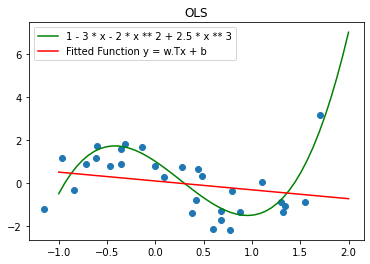
\includegraphics[scale=0.7]{singlevar_grad.png}
  \caption{Single Variable Regression - Gradient Descent (\texttt{epochs}=1000, \texttt{lr}=1e-2)}
\end{figure}
\begin{figure}[H]
  \centering
  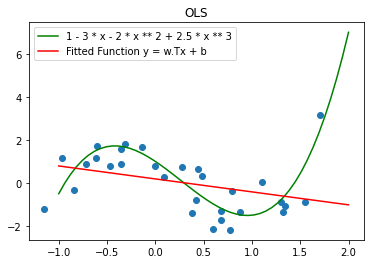
\includegraphics[scale=0.7]{singlevar_closedform.png}
  \caption{Single Variable Regression - Closed Form}
\end{figure}

\subsubsection{}
As mentioned in description of the question (point 5), the error function (mse) is convex and has just one minimum. \\
By using the closed form, we get the point corresponding to minimum mse error. As we compute the parameters based on training data, the training loss is minimum at this point. \\
Therefore, training loss for solution of \verb!singlevar_grad()! can never be strictly less than that of the solution obtained by \verb!singlevar_closedform()!.


\newpage
\section{OLS and Ridge Regression}
To avoid confusion in lab part where we should not regularize the bias term, I am considering the bias to be separate for now, i.e. apart from $W$ the weights to be learnt, we also have to learn $b$ the bias term. \\

Notation: \\
$\mathbf{X}$ is $N \times d$ matrix, \\
$\mathbf{Y}$ is $N \times 1$ vector, \\
$\hat{\mathbf{Y}}$ is $N \times 1$ vector, \\
$\mathbf{1_N}$ is $N \times 1$ vector (all 1s), \\
$\mathbf{W}$ is $d \times 1$ vector, \\
$\mathbf{x_i}$ is $d \times 1$ vector (i$^\text{th}$ observed sample), \\
$y_i$ is scalar (i$^\text{th}$ observed output), \\
$w_i$ is scalar (weight for i$^\text{th}$ feature), \\
$b$ is scalar.

\subsection{CS337: Theory}
\subsubsection{}
$\hat{\mathbf{Y}} = \mathbf{X} \mathbf{W} + b \mathbf{1_N}$, where $\mathbf{W}$ and $b$ are learnt from the given $N$ samples (which may be noisy).

\subsubsection{}
Assuming that partial derivative is $1 \times d$ row vector (numerator layout).
\begin{equation*}
  \begin{aligned}
    mse(\mathbf{W},b)                                      & = \frac{1}{N} \sum_{i=1}^N ((\mathbf{W}^T \mathbf{x_i} + b) - y_i)^2                                     \\
    \frac{\partial mse(\mathbf{W},b)}{\partial \mathbf{W}} & = \frac{1}{N} \sum_{i=1}^N 2 \ ((\mathbf{W}^T \mathbf{x_i} + b) - y_i) \ \mathbf{x_i}^T                  \\
                                                           & = \frac{2}{N} \sum_{i=1}^N (\mathbf{W}^T \mathbf{x_i} + b - y_i) \ \mathbf{x_i}^T                        \\
                                                           & = \frac{2}{N} \ \text{dot}(\text{dot}(\mathbf{X}, \mathbf{W}) + b \mathbf{1_N} - \mathbf{Y}, \mathbf{X}) \\
    \frac{\partial mse(\mathbf{W},b)}{\partial b}          & = \frac{1}{N} \sum_{i=1}^N 2 \ ((\mathbf{W}^T \mathbf{x_i} + b) - y_i)                                   \\
                                                           & = \frac{2}{N} \sum_{i=1}^N (\mathbf{W}^T \mathbf{x_i} + b - y_i)                                         \\
                                                           & = \frac{2}{N} \ \text{sum}(\text{dot}(\mathbf{X}, \mathbf{W})  + b \mathbf{1_N} - \mathbf{Y})
  \end{aligned}
\end{equation*}

\subsubsection{}
Assuming that partial derivative is $1 \times d$ row vector (denominator layout).
\begin{equation*}
  \begin{aligned}
    mse(\mathbf{W},b)                                      & = \lambda || \mathbf{W} ||_2^2 + \frac{1}{N} \sum_{i=1}^N ((\mathbf{W}^T \mathbf{x_i} + b) - y_i)^2                               \\
    \frac{\partial mse(\mathbf{W},b)}{\partial \mathbf{W}} & = 2 \lambda \mathbf{W}^T + \frac{1}{N} \sum_{i=1}^N 2 \ ((\mathbf{W}^T \mathbf{x_i} + b) - y_i) \ \mathbf{x_i}^T                  \\
                                                           & = 2 \lambda \mathbf{W}^T + \frac{2}{N} \sum_{i=1}^N (\mathbf{W}^T \mathbf{x_i} + b - y_i) \ \mathbf{x_i}^T                        \\
                                                           & = 2 \lambda \mathbf{W}^T + \frac{2}{N} \ \text{dot}(\text{dot}(\mathbf{X}, \mathbf{W}) + b \mathbf{1_N} - \mathbf{Y}, \mathbf{X}) \\
    \frac{\partial mse(\mathbf{W},b)}{\partial b}          & = \frac{1}{N} \sum_{i=1}^N 2 \ ((\mathbf{W}^T \mathbf{x_i} + b) - y_i)                                                            \\
                                                           & = \frac{2}{N} \sum_{i=1}^N (\mathbf{W}^T \mathbf{x_i} + b - y_i)                                                                  \\
                                                           & = \frac{2}{N} \ \text{sum}(\text{dot}(\mathbf{X}, \mathbf{W})  + b \mathbf{1_N} - \mathbf{Y})
  \end{aligned}
\end{equation*}

\subsubsection{}
Closed form of OLS is $\mathbf{W} = (\mathbf{X}^T \mathbf{X})^{-1} \mathbf{X}^T \mathbf{Y}$. \\
This closed form is not applicable when $\mathbf{X}^T \mathbf{X}$ is not invertible (is singular). \\
This happens when $\mathbf{X}$ is not full column rank, i.e. the columns (features) of $\mathbf{X}$ are linearly dependent. \\
We don't have a unique solution and therefore can't have a closed form. \\
We actually have infinite solutions (of $\mathbf{W}$). \\
(We can't have no solutions of OLS as it is a minimization problem) \\
Gradient descent therefore would converge towards these solutions. \\
(Depending on the starting point, it would descent to one of these solutions)

\newpage
\subsection{CS335: Lab}
\subsubsection{}
Code for the functions \verb!mse_multi_var()! and \verb!mse_regularized()! updated in notebook.

\subsubsection{}
Code for the functions \verb!multivar_grad()! and \verb!multivar_closedform()! updated in notebook.
\begin{figure}[H]
  \centering
  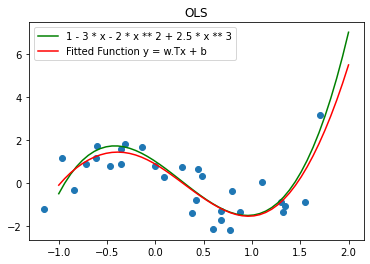
\includegraphics[scale=0.7]{multivar_grad.png}
  \caption{Multi Variable Regression - Gradient Descent (\texttt{epochs}=1000, \texttt{lr}=1e-1)}
\end{figure}
\begin{figure}[H]
  \centering
  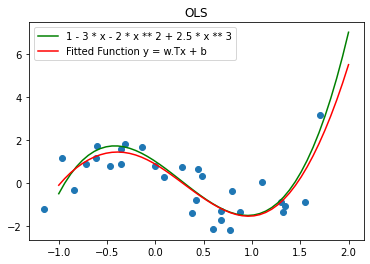
\includegraphics[scale=0.7]{multivar_closedform.png}
  \caption{Multi Variable Regression - Closed Form}
\end{figure}

\subsubsection{}
Code for the functions \verb!multivar_reg_grad()! and \verb!multivar_reg_closedform()! updated in notebook.
\begin{figure}[H]
  \centering
  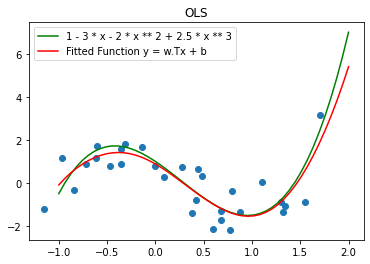
\includegraphics[scale=0.7]{multivar_reg_grad.png}
  \caption{Regularization - Gradient Descent (\texttt{epochs}=1000, \texttt{lr}=1e-1, \texttt{lamda}=0.001)}
\end{figure}
\begin{figure}[H]
  \centering
  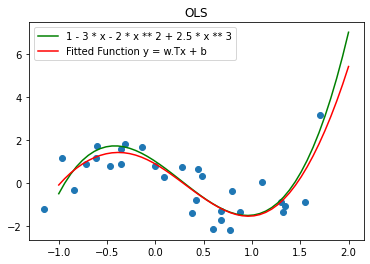
\includegraphics[scale=0.7]{multivar_reg_closedform.png}
  \caption{Regularization - Closed Form (\texttt{lamda}=0.001)}
\end{figure}


\newpage
\section{Bayesian Linear Regression}

\subsection{CS337: Theory}
\subsubsection{}
\begin{equation*}
  \begin{aligned}
    p(w) & = \frac{1}{\sqrt{2 \pi}} \exp \bigg( -\frac{(w - \mu_0)^2}{2} \bigg)
  \end{aligned}
\end{equation*}

\subsubsection{}
\begin{equation*}
  \begin{aligned}
    p(y | x; w) & = \frac{1}{\sqrt{2 \pi}} \exp \bigg( -\frac{(y - wx)^2}{2} \bigg)
  \end{aligned}
\end{equation*}

\subsubsection{}
\begin{equation*}
  \begin{aligned}
    p(\mathcal{D}; w) & = \prod_{i=1}^N \frac{1}{\sqrt{2 \pi}} \exp \bigg( -\frac{(y_i - wx_i)^2}{2} \bigg) \\
                      & = (2 \pi)^{-N/2} \exp \bigg( -\frac{\sum_{i=1}^N (y_i - wx_i)^2}{2} \bigg)
  \end{aligned}
\end{equation*}

\subsubsection{}
\begin{equation*}
  \begin{aligned}
    p(w | \mathcal{D})      & = \frac{p(\mathcal{D} | w) p(w)}{\int_{-\infty}^{\infty} p(\mathcal{D} | w) p(w) dw}           \\
    p(\mathcal{D} | w) p(w) & = (2 \pi)^{-(N+1)/2} \exp \bigg( -\frac{(w - \mu_0)^2 + \sum_{i=1}^N (y_i - wx_i)^2}{2} \bigg) \\
  \end{aligned}
\end{equation*}

\subsubsection{}
\begin{equation*}
  \begin{aligned}
    p(w | \mathcal{D}) & \propto \exp \bigg( -\frac{(w - \mu_0)^2 + \sum_{i=1}^N (y_i - wx_i)^2}{2} \bigg) \\
  \end{aligned}
\end{equation*}

\subsubsection{}
\begin{equation}
  \begin{aligned}
    \label{eq1}
    p(w | \mathcal{D}) & \propto \exp \bigg( -\frac{w^2 (1 + \sum_i x_i^2) - 2w(\mu_0 + \sum_i x_i y_i) + (\mu_0^2 + \sum_i y_i^2)}{2} \bigg) \\
  \end{aligned}
\end{equation}

\subsubsection{}
\begin{equation}
  \begin{aligned}
    \label{eq2}
    p(w | \mathcal{D}) & = \mathcal{N}(\mu_N, \sigma_N^2) \propto \exp \bigg( -\frac{(w - \mu_N)^2}{2 \sigma_N^2} \bigg)                                 \\
    p(w | \mathcal{D}) & \propto \exp \bigg( -\frac{w^2 (\frac{1}{\sigma_N^2}) - 2w (\frac{\mu_N}{\sigma_N^2}) + (\frac{\mu_N^2}{\sigma_N^2})}{2} \bigg) \\
  \end{aligned}
\end{equation}

\subsubsection{}
Comparing \eqref{eq1} and \eqref{eq2}, \\
\begin{equation*}
  \begin{aligned}
    \sigma_N^2 & = \frac{1}{1 + \sum_i x_i^2}                                     \\
    \mu_N      & = (\mu_0 + \sum_i x_i y_i) \sigma_N^2                            \\
               & = \frac{\mu_0 + \sum_i x_i y_i}{1 + \sum_i x_i^2} & (= w^*_{BE})
  \end{aligned}
\end{equation*}

\subsubsection{}
As $N \to \infty$, $\sum_i x_i^2 \gg 1$ and $\sum_i x_i y_i \gg \mu_0$. \\
$\sigma_N^2 \to \dfrac{1}{\sum_i x_i^2} \to 0$ ($x_i$s are iid, so $\sum_i x_i^2$ can never be convergent)\\
$\mu_N \to \dfrac{\sum_i x_i y_i}{\sum_i x_i^2} = \dfrac{\sum_i x_i (w_{\text{true}} x_i + \epsilon_i)}{\sum_i x_i^2} \to w_{\text{true}}$ ($\epsilon_i \sim \mathcal{N}(0, 1)$ and $E[y_i] = w_{\text{true}} x_i$)

\subsubsection{}
As we sample more and more data, we get more confident about the estimated value of $w$, and thus the variance $(\sigma_N^2)$ tends to zero, i.e. our estimate for $w$ is converging. \\
Also, we converge towards the true value as data starts to dominate over the prior information, thus the mean $(\mu_N)$ tends towards the $w_{\text{true}}$.

\subsection{MLE Estimate}
\subsubsection{}
\begin{equation*}
  \begin{aligned}
    w^* & = \argmax_w \ p(\mathcal{D}; w)                                                                                                            \\
        & = \argmax_w \ (2 \pi)^{-N/2} \exp \bigg( -\frac{\sum_{i=1}^N (y_i - wx_i)^2}{2} \bigg)                                                     \\
        & = \argmax_w \ \exp \bigg( -\frac{\sum_{i=1}^N (y_i - wx_i)^2}{2} \bigg)                                                                    \\
        & = \argmax_w \ -\frac{\sum_{i=1}^N (y_i - wx_i)^2}{2}                                   & \text{(ln is monotonically increasing function})  \\
        & = \argmin_w \ \sum_{i=1}^N (y_i - wx_i)^2                                              & \text{(-2x is monotonically decreasing function}) \\
  \end{aligned}
\end{equation*}
\begin{equation*}
  \begin{aligned}
     & \frac{d}{dw} \bigg( \sum_{i=1}^N (y_i - wx_i)^2 \bigg) \bigg\vert_{w=w^*} = 0 \implies 2 \bigg( \sum_{i=1}^N (y_i - w^* x_i) x_i \bigg) = 0 \\
     & w^* = \frac{\sum_i x_i y_i}{\sum_i x_i^2} \ (= w^*_{MLE})
  \end{aligned}
\end{equation*}

\subsubsection{}
$\lim_{N \to \infty} w^*_{BE} = w^*_{MLE} = \dfrac{\sum_i x_i y_i}{\sum_i x_i^2}$. \\
For infinite data, the prior becomes insignificant. \\
Maximum Likelihood Estimate (MLE) and Bayesian Estimate (BE) are equivalent and both converge towards the true value $w_{\text{true}}$.

\subsection{CS335: Lab}
\subsubsection{}
Code for the function \verb!bayesion_lr()! updated in notebook.
\begin{figure}[H]
  \centering
  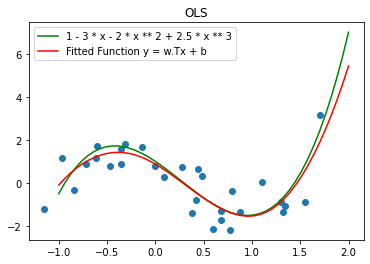
\includegraphics[scale=0.7]{bayesion_lr.png}
  \caption{Bayesian Linear Regression - Closed Form (\texttt{sigma}=0.1)}
\end{figure}

\subsubsection{}
In Closed form of OLS, we might have to invert a non-invertible matrix. $X^T X$ would be non-invertible when features aren't linearly independent. \\
Here, we take inverse of $X^T X + \lambda I$ (reminds of ridge regression). Even if we have features which aren't linearly independent, $X^T X + \lambda I$ would be invertible due to presence of $I$ which is a full rank matrix.


\newpage
\section{Conclusion}
Comparing the seven methods for the assignment problem:
\begin{enumerate}
  \item \textbf{Single Variable OLS Regression Gradient Descent} \\
        Gradient Descent can be slow; \\
        Need to set hyper-parameters - epochs and learning rate; \\
        Not a nice fit (Validation error approx 0.14)
  \item \textbf{Single Variable OLS Regression Closed Form} \\
        Closed form computation is fast; \\
        No hyper-parameters; \\
        Not a nice fit (Validation error approx 0.14)
  \item \textbf{Multi Variable OLS Regression Gradient Descent} \\
        Gradient Descent can be slow; \\
        Need to set hyper-parameters - epochs and learning rate; \\
        Nice fit (Validation error approx 0.03); \\
        Can give solution when the features aren't linearly independent
  \item \textbf{Multi Variable OLS Regression Closed Form} \\
        Closed form computation is fast; \\
        No hyper-parameters; \\
        Nice fit (Validation error approx 0.03); \\
        Can't give solution when the features aren't linearly independent
  \item \textbf{Multi Variable Regularized (Ridge) Regression Gradient Descent} \\
        Gradient Descent can be slow; \\
        Need to set hyper-parameters - lambda, epochs and learning rate; \\
        Nice fit (Validation error approx 0.03); \\
        Can give solution when the features aren't linearly independent
  \item \textbf{Multi Variable Regularized (Ridge) Regression Closed Form} \\
        Closed form computation is fast; \\
        Need to set hyper-parameter - lambda; \\
        Nice fit (Validation error approx 0.03); \\
        Can give solution when the features aren't linearly independent
  \item \textbf{Multi Variable Bayesian Regression Closed Form} \\
        Closed form computation is fast; \\
        Need to set hyper-parameter - prior and sigma; \\
        Nice fit (Validation error approx 0.03); \\
        Can give solution when the features aren't linearly independent
\end{enumerate}

Only method which doesn't require hyper-parameters and gives a good fit is Method 4 - Multi Variable OLS Regression Closed Form. However, it fails to give a solution when the features aren't linearly independent. \\

Now that we have to set some hyper-parameter, we can decide the method based on number of features. \\
In all closed forms, we compute inverse of a $d \times d$ matrix. The complexity of this computation is $\mathcal{O}(d^3)$. Thus, this method might be infeasible for large number of features. \\

For large number of features, if the features are known to be linearly independent then we can use Method 3 - Multi Variable OLS Regression Gradient Descent, else we should prefer Method 5 - Multi Variable Regularized (Ridge) Regression Gradient Descent (this would remove redundant features). \\

For small number of features (like in this assignment), closed form solutions would be faster and more accurate. If we have some prior for the parameter then we can use Method 7 - Multi Variable Bayesian Regression Closed Form or we can try different lambdas for Method 6 - Multi Variable Regularized (Ridge) Regression Closed Form. \\

For this assignment, I prefer Method 6 - Multi Variable Regularized (Ridge) Regression Closed Form.

\end{document}
